\documentclass{amia}
\usepackage{graphicx}
\usepackage[labelfont=bf]{caption}
\usepackage[superscript,nomove]{cite}
\usepackage{color}
\usepackage{multirow}
\renewcommand*{\thefootnote}{\fnsymbol{footnote}}

\begin{document}

\title{Predicting Success of Clinical Interviews via Probabilistic Modeling of Patient-Provider Communication Sequences}

\author{Alexander Kotov, PhD$^{1}$\footnote[1]{Authors provided equal contribution. \label{footnote1}}, Mehedi Hasan, BS$^{1}$\textsuperscript{\ref{footnote1}}, April Idalski Carcone, PhD$^{2}$, Ming Dong, PhD$^{1}$, Sylvie Naar, PhD$^{2}$}

\institutes{
$^1$Department of Computer Science,  
$^2$Department of Family Medicine and Public Health Sciences, School of Medicine, Wayne State University, Detroit, Michigan\\
}

\maketitle

\noindent{\bf Abstract}
\textit{The problem of analyzing temporally ordered observation sequences to make predictions related to the outcome of the processes that generated these sequences arises in many domains of healthcare informatics. In this paper, we focus on patient-provider communication sequences in the context of clinical interviews and propose two methods, based on Markov chain and Hidden Markov Model, for predicting the likelihood of eliciting a particular type of patient behavioral response based on an observed sequence of patient-provider exchanges.  Our method achieved 75.32\% and 79.89\% F-measure for natural sequences and 97.36\% and 96.99\% F-measure for alternating sequences in predicting the outcome of motivational interviews with obese adolescents using first and second order Markov Chain and Hidden Markov Model, respectively. The proposed method can be used to automatically identify the most effective communication strategies in motivational interviews, which significantly decreases the effort required to develop effective interventions to address many public health conditions.}

\section*{Introduction}
Data in the form of temporally ordered sequences of discrete or continuous observations (e.g., symbolic sequences such as notes in patient EHR, diagnostic codes, protein or DNA sequences or continuous time series, such as ECG measurements) arise in various domains of health informatics. The order of observations in a sequence is challenging to capture using features, which makes sequence classification a more challenging task than traditional classification. In general, sequence classification methods can be divided into three  categories: feature-based, distance metric-based and model-based method. Feature-based classification methods transform a sequence into a feature vector and apply a standard supervised learning algorithm, such as support vector machine \cite{leslie2004fast} or decision tree \cite{chuzhanova1998feature}. Shapelet \cite{ye2009time} and pattern \cite{kudenko1998feature, lesh1999mining} based techniques as well as hierarchical approaches \cite{nallam2016effective} have been proposed instead of standard classifiers as well. Distance-based methods measure the similarity between sequences to determine the quality of classification. The most commonly used distance function is Euclidian distance \cite{keogh2003need} with Dynamic Time Wrapping \cite{keogh2000scaling} used for more flexible matching in time series data. The third type of sequence classification methods, first create a probabilistic model of a sequence, such as Hidden Markov Model \cite{rabiner1989tutorial} (HMM).

Sequence classification has a broad range of real word applications from genomics and health informatics to finance and anomaly detection. In genomics research, sequence classification is widely used to classify protein and text sequence data \cite{yakhnenko2005discriminatively} and detect the function of new proteins \cite{deshpande2002evaluation}. In health informatics, ECG measurements are considered as multi-dimensional time series and are used to classify individuals as healthy or having a heart disease \cite{wei2006semi}. Sequence classification is also used for anomaly detection such as abnormal access to systems \cite{lane1999temporal} and malware \cite{drew2017polymorphic}.    

In this paper, we direct our focus towards patient-provider communication sequences in the context of clinical interviews. Specifically, we focus on the transcripts of Motivational Interviews (MI) with obese adolescents and their caregivers. Childhood obesity is a serious public health concern in the United States and worldwide. Recent estimates indicate that approximately one third (31.8\%) of US children age 2-19 years are overweight and 16.9\% are obese \cite{ogden2012prevalence}. Adolescents who are obese likely continue to be obese in adulthood and have a greater risk of heart disease, type 2 diabetes, stroke, cancer, and osteoarthritis \cite{general2010surgeon}. One approach to effective obesity intervention is Motivational Interviewing, an evidence-based counseling technique to increase intrinsic motivation and self-efficacy for health-related behavior change. The goal of MI counseling session is to encourage patients to explore their own desires, ability, reasons, need for and commitment to the targeted behavior change. These statements, referred to as ``change talk'' (or CT), consistently predict actual behavior change that can be sustained for as long as 34 months after an interview. However, the ability of counselors to consistently elicit this type of patient communication requires knowledge of effective communication strategies for a variety of patients, which can only be obtained through analysis of a large number of annotated interviews. Since manual annotation and examination of transcripts is a very time-consuming process, tailoring of MI interventions to particular populations can take years. Therefore, there is a need for informatics-based methods to facilitate the development of effective MI-based interventions, in general, and theoretically-grounded computational models to explore the mechanisms of MI's efficacy, in particular.  

Our research addresses this problem from multiple angles. In our previous work \cite{kotov2015interpretable, hasan2016study}, we explored several machine learning methods for automatic annotation of clinical interview fragments with a specialized codebook containing a large number of patient and provider behavior codes \cite{carcone2013provider}. In this work, we propose probabilistic methods to identify patient-provider communication sequences that are likely to elicit the desired patient behavioral response (i.e. change talk or commitment language) and to dynamically estimate the likelihood of observing this desired response at any point during a clinical interview based on all coded previous patient-provider communication exchanges in the same interview. While there have been some previous qualitative studies of patient-provider dialog in a clinical setting \cite{eide2004physician}, there have been no previous work on computational modeling of annotated patient-provider communication (PPC) exchanges and predicting a desired patient behavior in a context of motivational interviews.   

\section*{Methods}
\subsection*{\textit{Data collection}}
The experimental dataset for this work was constructed from the transcripts of 37 motivational interviews, which include a total of 11,353 segmented and annotated utterances. Each transcript consists of a counselor-adolescent and a counselor-caregiver session. Since the ultimate goal of a motivational interview is to increase the desire and ability of adolescents for a targeted behavior change, we considered only communication sequences from counselor-adolescent sessions and disregarded all communication sequences from counselor-caregiver sessions. The utterances were annotated based on MYSCOPE codebook \cite{carcone2013provider}, which are grouped into the adolescent and counselor code groups. Utterances were divided into successful and unsuccessful communication sequences. Successful communication sequences result in positive change talk and commitment language (a special class of change talk) statements by an adolescent, while unsuccessful sequences are the ones that result in negative change talk or commitment language and the sequences, in which no change talk or commitment language statements occur. Out of 1072 observed sequences, 880 were positive and 192 were negative. Alternating communication sequences are sub-sequences of a natural communication sequence, in which two consecutive utterances cannot belong to the same speaker (i.e. a counselor behavior code has to be followed by an adolescent behavior code and vice versa). For example, 6 alternating sequences (\{C1, A1, C2, A3\}, \{C1, A1, C3, A3\}, \{C1, A1, C4, A3\}, \{C1, A2, C2, A3\}, \{C1, A2, C3, A3\} and \{C1, A2, C4, A3\}) can be created from a natural sequence \{C1, A1, A2, C2, C3, C4, A3\}, where adolescent and counselor codes are represented by A and C, respectively. A total of 18753 alternating sequences have been observed in experimental dataset, out of which 18139 were successful and 614 were unsuccessful ones. For each type of sequence (natural and alternating), one probabilistic model was trained using successful sequences and one model was train using unsuccessful sequences. Statistics of experimental dataset are presented in Table~\ref{tab:data_dist} and a fragment of an adolescent session transcript is presented in Table~\ref{tab:anno_examp}. \\

\begin{table}[h]
\centering
\caption{Statistics of experimental dataset. Sequence length is the number of behavior codes in it.}
\label{tab:data_dist}
  \begin{tabular}{|l|l|l|l|l|}
  \hline
   \textbf{Sequence type} & \textbf{Total sequences}  & \textbf{\# Successful sequences}  & \textbf{\# Unsuccessful sequences} & \textbf{Avg. length} \\ \hline      
Natural sequences & 1072 & 880 (82.09\%) & 192 (17.91\%) & 5.83 \\\hline
Alternating sequences & 18753 & 18139 (96.72\%) & 614 (3.28\%) & 12.89 \\\hline 
  \end{tabular}
\end{table} 

Annotation column in Table~\ref{tab:anno_examp} shows the sequence of behavior codes from top to bottom, where counselor starts with an open-ended question and gets positive feedback at the end. \\

\begin{table}[h]
\caption{Fragment of the annotated transcript of a dialogue between a counselor and an adolescent.}    
\label{tab:anno_examp}
\centering
\begin{tabular}{|l|p{3.6cm}|l|p{8cm}|}
\hline
Annotation  & Description & Speaker & Text \\\hline
331 &	Open-ended question, elicit change talk positive &	Counselor &	do you feel like making healthier choices for your snacks and your meals is something you would be able to do? mm-hmm meaning is that food available for you? \\\hline
117 &	Low Uptake, positive	& Adolescent &	Yes \\\hline
301 &	Structure Session	& Counselor &	okay and thats an important thing for us to think about cause i would not want to help you come up with a plan that you would not be able to do without somebody else help so the last part of your plan is how somebody could be supportive to you meaning how they can help you be successful and so we should choose somebody who you feel like is around often enough \\\hline
112 &	Change Talk positive	& Adolescent &	my um aunt \\\hline
301 &	Structure Session	& Counselor &	okay so lets stick something my aunt can do \\\hline
112 &	Change Talk positive &	Adolescent &	she could when i am doing when i am eating something that i should i could not be eating but so i can choose something healthy she could tell me not to eat it \\\hline
309 &	Affirm, low &	Counselor &	okay that sounds like a really great suggestion \\\hline
\end{tabular}
\end{table}  

\subsection*{\textit{Prediction method}}

Generally, a sequence is a temporally ordered set of events. In this study, an event is a behavior code that also has a symbolic representation, such as 117 $LUP+$ (low uptake, positive), 331 $OQ-ECT+$ (open-ended question, elicit change talk positive), etc.  Given a sequence of behavior codes $S_i = \{c_1, c_2,...,c_n\}$ representing patient-provider communication exchanges during some part of a motivational interview, the task of predicting interview success can be viewed as sequence classification. Given a set of class labels $L = \{l_1, l_2,...,l_m\}$ (in our case, the labels are ``successful'' and ``unsuccessful'' motivational interview), a sequence classifier $C$ learns a function $S_i \to l_i, l_i \in L$ that maps a sequence $S_i$ into a class label $l_i \in L$.

Our proposed prediction method consists of two steps. In the first step, we model successful and unsuccessful patient-provider interactions using first- and second-order Markov Chain (MC) and Hidden Markov Model (HMM), which are popular probabilistic models for discrete observation sequences with finite vocabulary. Although HMM was originally developed for speech recognition \cite{rabiner1989tutorial}, it is one of the most widely used methods for sequence modeling \cite{mutsam2016maximum, eickeler1998hidden, srivastava2007hmm, won2004training, chai2001folk}.

\textbf {Markov Chain (MC)} is a stochastic model for randomly changing systems, which assumes that the next state of a system only depends on its current state and not on its past states (Markov property). Generally, this assumption enables reasoning and computation with the models that would otherwise be intractable. For the sequential analysis, we built two Markov models $M$ and $\overline{M}$ summarizing provider strategies and patient responses in case of successful ($M$) and unsuccessful ($\overline{M}$) motivational interviews. A Markov model $M$ can be represented as a weighted directed graph $G = (V, E, p)$, in which:

\begin{itemize}
\item $V = \{CML+, CHT+, CHT-, T-AMB, CCT, BLT, LUP+, LUP-, HUP-W, ...\}$ is a set of vertices, consisting of adolescent and counselor MI behavior codes;
\item $E \subseteq V \times V$ is a set of edges corresponding to posssible transitions from one MI behavior code to the other in a sequence;
\item $p_M:E\rightarrow[0...1]$ is a function that assigns probability $p(c_i|c_j)$ to an edge between the MI behavior codes $c_i$ and $c_j$ based on maximum likelihood estimator:

\begin{equation}
P_M(c_j|c_i) = \frac{n_{c_i,c_j}}{n_{c_i}}
\end{equation}

\end{itemize}

where $n_{c_i,c_j}$ and $n_{c_i}$ are the number of times a transition between the MI behavior codes $c_i$ and $c_j$ and the code $c_i$ has been observed in the training data. Given a Markov model $M$ (such that $S\subseteq V$), the probability that a sequence of MI behavior codes $S = \{C_1,...,C_N\}$ has been generated from a Markov model $M$ is:

\begin{equation}
P_M(S) = \prod_{i=2}^N p_M(c_i|c_1,\dots,c_{i-1})=\prod_{i=2}^N p_M(c_i|c_{i-1})
\end{equation}

In the second step, we quantify the likelihood of success of a given motivational interview at a certain time point given a sequence of MI behavior codes $S$ observed prior to that point using the following formula:

\begin{equation}
p(S\rightarrow CML+) = \log\left(\frac{P_M(S)}{P_{\overline M}(S)}\right)= \sum_{i=2}^N \log p_M(c_i|c_{i-1})-\sum_{i=2}^N \log p_{\overline M}(c_i|c_{i-1})\label{eq:class}
\end{equation}

If $p(S\rightarrow CML+) > \delta $, where $\delta$ is an empirically determined threshold, the interview is predicted to result in positive change talk or commitment language. Tuning the proposed method on the training data involves experimentally determining the value of $\delta$, which results in the highest prediction F-measure with lower bias. Figure~\ref{fig:delta} illustrates the performance of Markov Chain-based prediction method by varying the value of $\delta$. As can be seen from Figure~\ref{fig:delta}, F-measure varies insignificantly, when $\delta $ is between -5 to -1, due to possible bias. However, F-score sharply decreases after $\delta = -0.9$. Thus, -0.9 is the optimal value of $\delta $, where F-measure is the highest with lower bias. 

\begin{figure}[htb!]
    \centering
    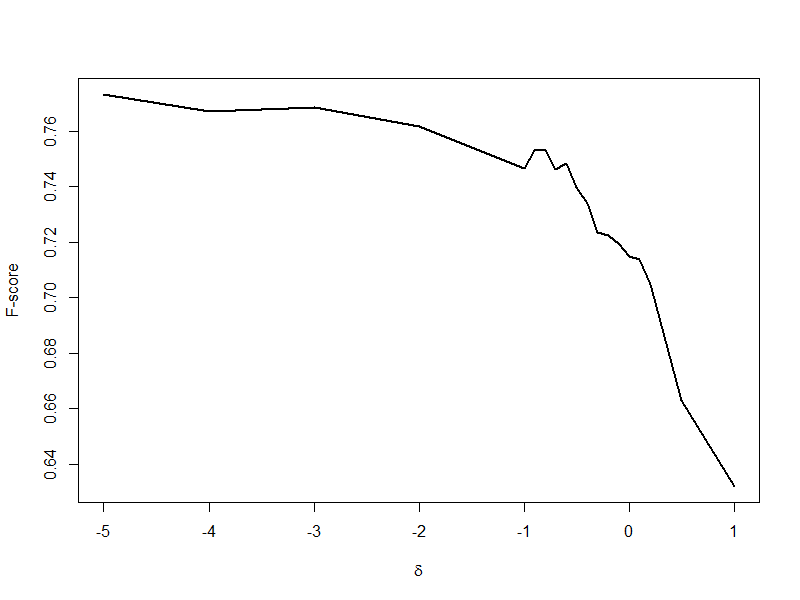
\includegraphics[width=0.70\textwidth]{figures/delta.png}
    \caption{\textbf{F-Measure of the proposed Markov model-based method by varying the value of $\delta$}.}
    \label{fig:delta}
\end{figure}

The Markov model we have discussed so far is referred to as the first-order MC, since it only considers immediately preceding behavior code when computing the state transition probabilities. A generalization of the first-order MC is the $k^{th}$ order MC, in which the transition probability to a particular state (symbol) $x_i$ is computed by looking at the k preceding states (symbols). Thus, $k^{th}$ order Markov chain will have $N^{k}$ states each associated with a sequence of k symbols. In our experiment, we also used second order Markov model. Hence, our model has $N^2$ states with transition probability matrix of size $N^2 \times N$.  

\textbf {Hidden Markov Model (HMM)} is a powerful tool for statistical modeling of processes varying in time. HMMs are widely used for sequence analysis because of their ability to incorporate dependencies among elements in sequence. HMM can be considered as a doubly embedded stochastic process with a process that is not observable (hidden process) and can only be observed through another stochastic process (observable process) that produces a sequence of observations. An HMM can be fully specified by the following quintuple: $\lambda = (N, M, A, B, \pi)$

\begin{itemize}
\item N is a number of hidden states in the model
\item M is a number of distinct observations symbols per state, i.e. the discrete vocabulary size
\item A is an $N\times N$ state transition probability distribution matrix $A = \{a_{ij}\}$
\item B is an $N\times M$ matrix $B = \{b_j(k)\}$ with observation symbol probability distribution for each state 
\item $\pi$ is the initial state distribution vector $\pi = \{\pi_i\}$
\end{itemize}

We exclude the structure parameters M and N to designate HMM using a compact notation: $\lambda = (A, B, \pi)$. The key difference between HMM and MC is that HMM requires specifying the number of hidden states as a model parameter and then the model deduces a sequence of hidden states that best explains the observations along with state transition probabilities and distributions of observation symbols for each state. The Baum-Welch algorithm was used to estimate the parameters of HMMs for successful and unsuccessful interviews using the corresponding training set, while the Viterbi algorithm was used to determine the most likely sequence of hidden states for a given sequence of observations. After assignment of hidden states, the log-likelihood of successful outcome can be estimated using Eq.~\ref{eq:class}. As in the case of MC, we also experimented with second-order HMM.   

\subsection*{\textit{Evaluation metrics}}
Performance of the proposed method was evaluated in terms of precision, recall, and F-measure using 5-fold cross-validation and weighted macro-averaging of these metrics over the folds. A true positive (TP) was counted when the method correctly classified a sequence into its actual class; a false positive (FP) was counted for a class when the method incorrectly classified a sequence into that class; a false negative (FN) for an actual class of sequence was counted when the method incorrectly classified the sequence into other class. Precision of a class was defined as the ratio of the numbers of correctly classified sequences and all sequences identified as belonging to that particular class by the classifier (i.e Precision = TP / (TP + FP)). Recall of a class was defined as the ratio between the numbers of correctly classified sequences and all sequences of that particular class in the gold standard (i.e. Recall = TP / (TP + FN)). F-measure is computed as the harmonic mean of precision and recall (i.e. 2 x Precision x Recall / (Precision + Recall)).   

\section*{Results}
Experimental evaluation of the proposed method is conducted on both natural sequences and alternating sequences. 

\subsection*{\textit{Predictive performance for natural PPC code sequences}}
Predictive performance summary of the proposed methods on natural sequences is presented in Table~\ref{tab:result_norm_seq}. Three major conclusions can be drawn from the results in Table~\ref{tab:result_norm_seq}. First, HMM-based method generally outperforms MC-based one across all metrics for natural sequences. Second, first-order HMM has the best performance in terms of precision (0.7980) and F-measure (0.7989), while second-order HMM achieves the highest recall (0.8449). Third,  it follows that second-order MC and HMM have lower precision and F-measure, but higher recall than first-order MC and HMM. In particular, precision and F-measure decrease by 6.74\% and 2.39\%, in case of MC, and by 7.27\% \& 2.09\%, in case of HMM, when going from first- to second-order models. In contrast, recall improves by 3\%--5\%, in case of both MC and HMM, when going from first- to second-order models. \\

\begin{table}[h]
\centering
\caption{Performance of MC and HMM for predicting success of natural patient-provider communication sequences. The largest value for each performance metric is highlighted in bold.}
\label{tab:result_norm_seq}
  \begin{tabular}{|l|l|l|l|l|l|}
  \hline
   \textbf{Model} & \textbf{Order}  & \textbf{Precision}  & \textbf{Recall} & \textbf{F-Measure}\\ \hline    
    
 \multirow{2}{*}{Markov Chain} & First order & 0.7387 & 0.7686 & 0.7532\\\cline{2-5}
 & Second order & 0.6889 & 0.7889 & 0.7352\\ \hline
 \multirow{2}{*}{Hidden Markov Model} & First order & \textbf{0.7980} & 0.8059 & \textbf{0.7989}\\ \cline{2-5}
 & Second order & 0.7400 & \textbf{0.8449} & 0.7822\\ \hline
 
  \end{tabular}
\end{table} 

\subsection*{\textit{Predictive performance for alternating PPC code sequences}}
Table~\ref{tab:result_alt_seq} summarizes predictive performance of the proposed methods on alternating sequences. These results indicate that second-order HMM had better recall than MC, achieving 97.13\% recall. Similar to the case of natural sequences, prediction method based on second-order HMM has the highest recall of 0.9713 among all models. However, different from natural sequences, second-order MC has the highest precision (0.9778) as well as the highest F-measure (0.9736). We also observed that second-order MC and HMM outperform first-order MC and HMM. Specifically, moving from first-order to second-order MC improves precision, recall and F-measure of the MI success prediction method by 0.01\%, 2.72\% and 1.37\%, respectively. Moving from first-order to second-order HMM improves precision, recall and F-measure of the MI success prediction method by 3.32\%, 4.30\% and 3.70\%, respectively.\\

\begin{table}[h]
\centering
\caption{Performance of MC and HMM for predicting success of natural patient-provider communication sequences. The largest value for each performance metric is highlighted in bold.}
\label{tab:result_alt_seq}
  \begin{tabular}{|l|l|l|l|l|l|}
  \hline
   \textbf{Model} & \textbf{Order}  & \textbf{Precision}  & \textbf{Recall} & \textbf{F-Measure}\\ \hline    
    
 \multirow{2}{*}{Markov Chain} & First order & 0.9777 & 0.9437 & 0.9604\\\cline{2-5}
 & Second order & \textbf{0.9778} & 0.9694 & \textbf{0.9736}\\ \hline
 \multirow{2}{*}{Hidden Markov Model} & First order & 0.9392 & 0.9313 & 0.9353\\ \cline{2-5}
 & Second order & 0.9704 & \textbf{0.9713} & 0.9699\\ \hline
  \end{tabular}
\end{table}

\subsection*{\textit{Impact of hidden states}}
While MC is a non-parametric method, HMM has an important parameter, the number of hidden states. A natural question is how does this parameter affect the performance of HMM-based prediction  method. Figure~\ref{fig:hidden-states} provides an answer to this question by illustrating the performance of the proposed method using HMMs of different order in terms of F-measure on different types of sequences. As follows from this Figure, in general, the number of states does not significantly impact the classification performance. All four models show their best performance when the number of states is between 4 and 8. 

Tables~\ref{tab:emission_matrix_s} and \ref{tab:emission_matrix_u} show patient-provider communication (PPC) codes with the highest probability in emission probability distributions associated with different states of HMMs trained on successful and unsuccessful interviews.\\

\begin{figure}[!htb]
    \centering
    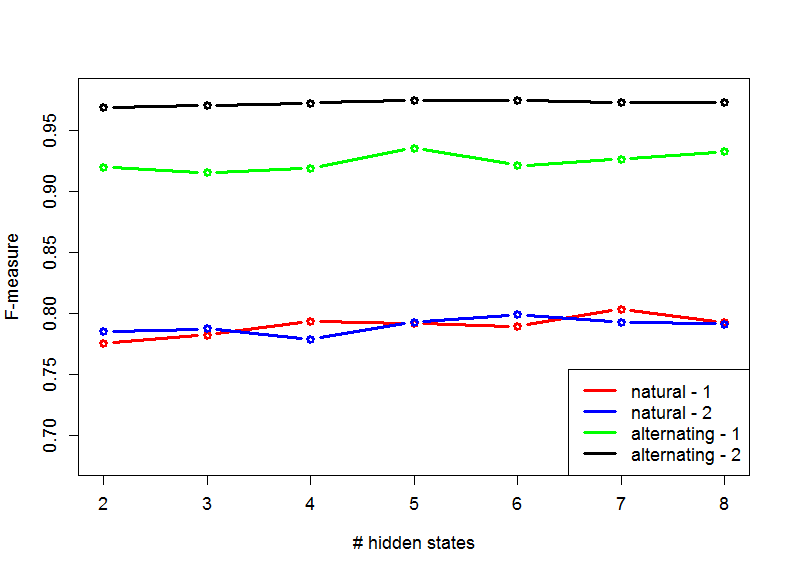
\includegraphics[width=0.70\textwidth]{figures/hidden-states.png}
    \caption{\textbf{Performance of the proposed method using HMMs of different order by varying the number of hidden states}.}
    \label{fig:hidden-states}
\end{figure}

\begin{table}[!htb]
\centering
\caption{PPC codes with the highest probability associated with different states of an HMM trained on successful interviews.}
\label{tab:emission_matrix_s}
  \begin{tabular}{|l|l|}
  \hline
   \textbf{State} & \textbf{Most likely PPC codes} \\\hline 
1 & SS, EA, R-CT+, OQ-ECT+, SUM-S, AF, R-CML+ \\\hline           
2 & LUP+, EA, OQ-ECT+, OQ-ECML+  \\\hline    
  \end{tabular}
\end{table} 

\begin{table}[!htb]
\centering
\caption{PPC codes with the highest probability associated with different states of an HMM trained on unsuccessful interviews.}
\label{tab:emission_matrix_u}
  \begin{tabular}{|l|l|}
  \hline
   \textbf{State} & \textbf{Most likely PPC codes} \\\hline     
1 & OQ-TBN, EA, R-CT+, AR, SUM-S, RBA-S, G-INFO+, R-CML+, OQ-ECT- \\\hline
2 & LUP+, OQ-ECT+, G-INFO+, CQ-EF, CHT-, HUP-O \\\hline
  \end{tabular}
\end{table} 

\subsection*{\textit{Common patterns}}
Table~\ref{tab:common_patterns} provides examples of typical PPC sequences that frequently appear in successful and unsuccessful motivational interviews. It can be seen that most successful patterns start with a summary of the discussion or open-ended/close-ended question. After that, if adolescents express positive change talk, the counselor immediately reflects on that to reinforce adolescent's intrinsic motivation about behavior change. On the other hand, providing information can lead to negative change talk, even in the cases when adolescents were showing positive tendency in their previous communication. This observation can be explained by adolescents quickly loosing focus when provided with general information that undermines their motivation. Analyzing such cases will allow the counselors to determine the general information that can be provided during the interviews. \\

\begin{table}[h]
\centering
\caption{Common patterns in successful and unsuccessful motivational interviews.}
\label{tab:common_patterns}
  \begin{tabular}{|l|l|}
  \hline
   \textbf{Type} & \textbf{Pattern} \\ \hline      
successful & 328 SUM-S: Summarize $\rightarrow $ 117 LUP+: Low Uptake, positive $\rightarrow $ 313 R-CML+: Reflect, \\ 
& commitment language positive $\rightarrow $ [positive commitment] \\\hline
successful & 307 SPT: Support $\rightarrow $ 117 LUP+: Low Uptake, positive $\rightarrow $ 313 R-CML+: Reflect, \\
& commitment language positive $\rightarrow $ [positive commitment] \\\hline
successful & 306 CQ-EF: Closed question, Elicit Feedback $\rightarrow $ 120 HUP-O: High Uptake, other \\
& $\rightarrow $ 313 R-CML+: Reflect, commitment language positive $\rightarrow $ [positive commitment] \\\hline
unsuccessful & 311 R-CT+: Reflect, change talk positive $\rightarrow $ 117 LUP+: Low Uptake, positive $\rightarrow $ 302 G-INFO+:  \\
& General Information, positive $\rightarrow $ [negative commitment] \\\hline
unsuccessful & 302 G-INFO+: General Information, positive $\rightarrow $ 117 LUP+: Low Uptake, positive $\rightarrow $  \\
& 302 G-INFO+: General Information, positive $\rightarrow $ [negative commitment] \\\hline
unsuccessful & 305 EA: Emphasize Autonomy $\rightarrow $ 117 LUP+: Low Uptake, positive $\rightarrow $ 302 G-INFO+:  \\
& General Information, positive $\rightarrow $ [negative commitment] \\\hline
  \end{tabular}
\end{table} 

\section*{Discussion}
By analyzing the experimental results of different communication sequence outcome prediction schemes proposed in this paper, we arrived at the following conclusions. First, using higher-order models results in better prediction accuracy compared to lower-order models, since higher-order models utilize larger context and can better capture different nuances of patient-provider communication. On the other hand, the number of states in higher-order Markov models grows exponentially with their order. Therefore, accurate estimation of transition probabilities requires much larger training set. Using smaller datasets will result in a sparsity problem, when many transitions are either not observed in the training set at all or observed only a few times, leading to missing or potentially inaccurate probability estimates. Obtaining large training sets cannot be easily accomplished in many domains, including motivational interviewing. In this study, we found out that using second-order Markov models is a reasonable trade-off between efficiency and accuracy.  

Second, the overall predictive performance of HMM is substantially better than MC for both types of sequences. In particular, HMM-based method achieves near-human accuracy for predicting the success of motivational interviews. This indicates that hidden states in HMM are able to capture the structure of discourse in motivational interviews by grouping together the codes that correspond to different cognitive states of adolescents during motivational interviews, which reflect the overall progression of the interviews. This allows to reduce the dimensionality of codes in PPC sequences and consequently improve both precision and recall of the prediction method. 

Third, converting natural PPC communication sequences to alternating ones results in better performance for all configurations of the proposed method. This indicates that alternating sequences emphasize the dependencies between the pairs of patient and provider codes, which results in more accurate estimates of the corresponding conditional probabilities. Better estimates of parameters in Markov models of successful and unsuccessful interviews are propagated to the next step, where they are aggregated into predictions for the entire sequence. This allows to achieve a dramatic improvement in the prediction accuracy of the method. 

Fourth, the proposed method can be used to identify the most effective communication strategies at eliciting a particular type of behavioral response. Awareness of these strategies by researchers can significantly decrease the time and effort required to develop effective interventions to address many public health conditions, such as childhood obesity, and tailor these interventions to particular patient cohorts. Awareness of these strategies by the counselors can lead to greater success rate of motivational interviews.     
 
\section*{Conclusion}
In this paper, we proposed a method based on Markov Chain and Hidden Markov Model for predicting the success of motivational interviews. We found out that individual patient-provider communication exchanges are highly indicative of the overall progression and future trajectory of clinical interviews and can be used to predict their overall success. Our proposed method can facilitate motivational interviewing researchers in establishing causal relationships between different communication strategies and the desired behavioral outcomes during the  interviews without resource intensive manual qualitative analysis of interview transcripts. Our proposed method can also help identify specific patterns that are common to successful and unsuccessful motivational interviews, which can also directly inform clinical practice. This work also has broad implications for qualitative public health research by providing a formal theoretically-grounded computational mechanism to facilitate the development of effective behavioral interventions.

\section*{Acknowledgments}
This study was supported by an R21 grant DK108071 from the NIH. We would like to thank the student assistants in the Department of Family Medicine and Public Health Sciences at Wayne State University School of Medicine for their help with transcribing the recordings of motivational interviews. 
\pagebreak

\bibliographystyle{vancouver}
\bibliography{references}

\end{document}